%%%%%%%%%%%%%%%%%%%%%%%%%%%%%%%%%%%%%%%%%%%%%%%%%%%%%%%%%%%%%%%%%%%%%%%%
% Plantilla TFG/TFM
% Escuela Politécnica Superior de la Universidad de Alicante
% Realizado por: Jose Manuel Requena Plens
% Contacto: info@jmrplens.com / Telegram:@jmrplens
%%%%%%%%%%%%%%%%%%%%%%%%%%%%%%%%%%%%%%%%%%%%%%%%%%%%%%%%%%%%%%%%%%%%%%%%

\chapter{Metodología}
\label{metodologia}

El desarrollo de este proyecto respeta tanto el proceso de desarrollo \textit{Software} como el ciclo de vida de proyectos de \textit{Ciencia de Datos}, por lo que se ha dividido en varias fases acontecidas que definiremos a continuación en base a la planificación mediante un \textit{Diagrama de Gantt}:

\section{Diagrama de Gantt}

    Un diagrama de Gantt es una herramienta que ayuda a visualizar las fases de evolución de un proyecto. Genera una vista global de cada una de las fases desarrolladas y su estimación temporal. A continuación se muestra el diagrama de Gantt realizado respecto a cada una de las fases de este proyecto \ref{GranttImage}.
    \begin{figure}[H]
        \centering
        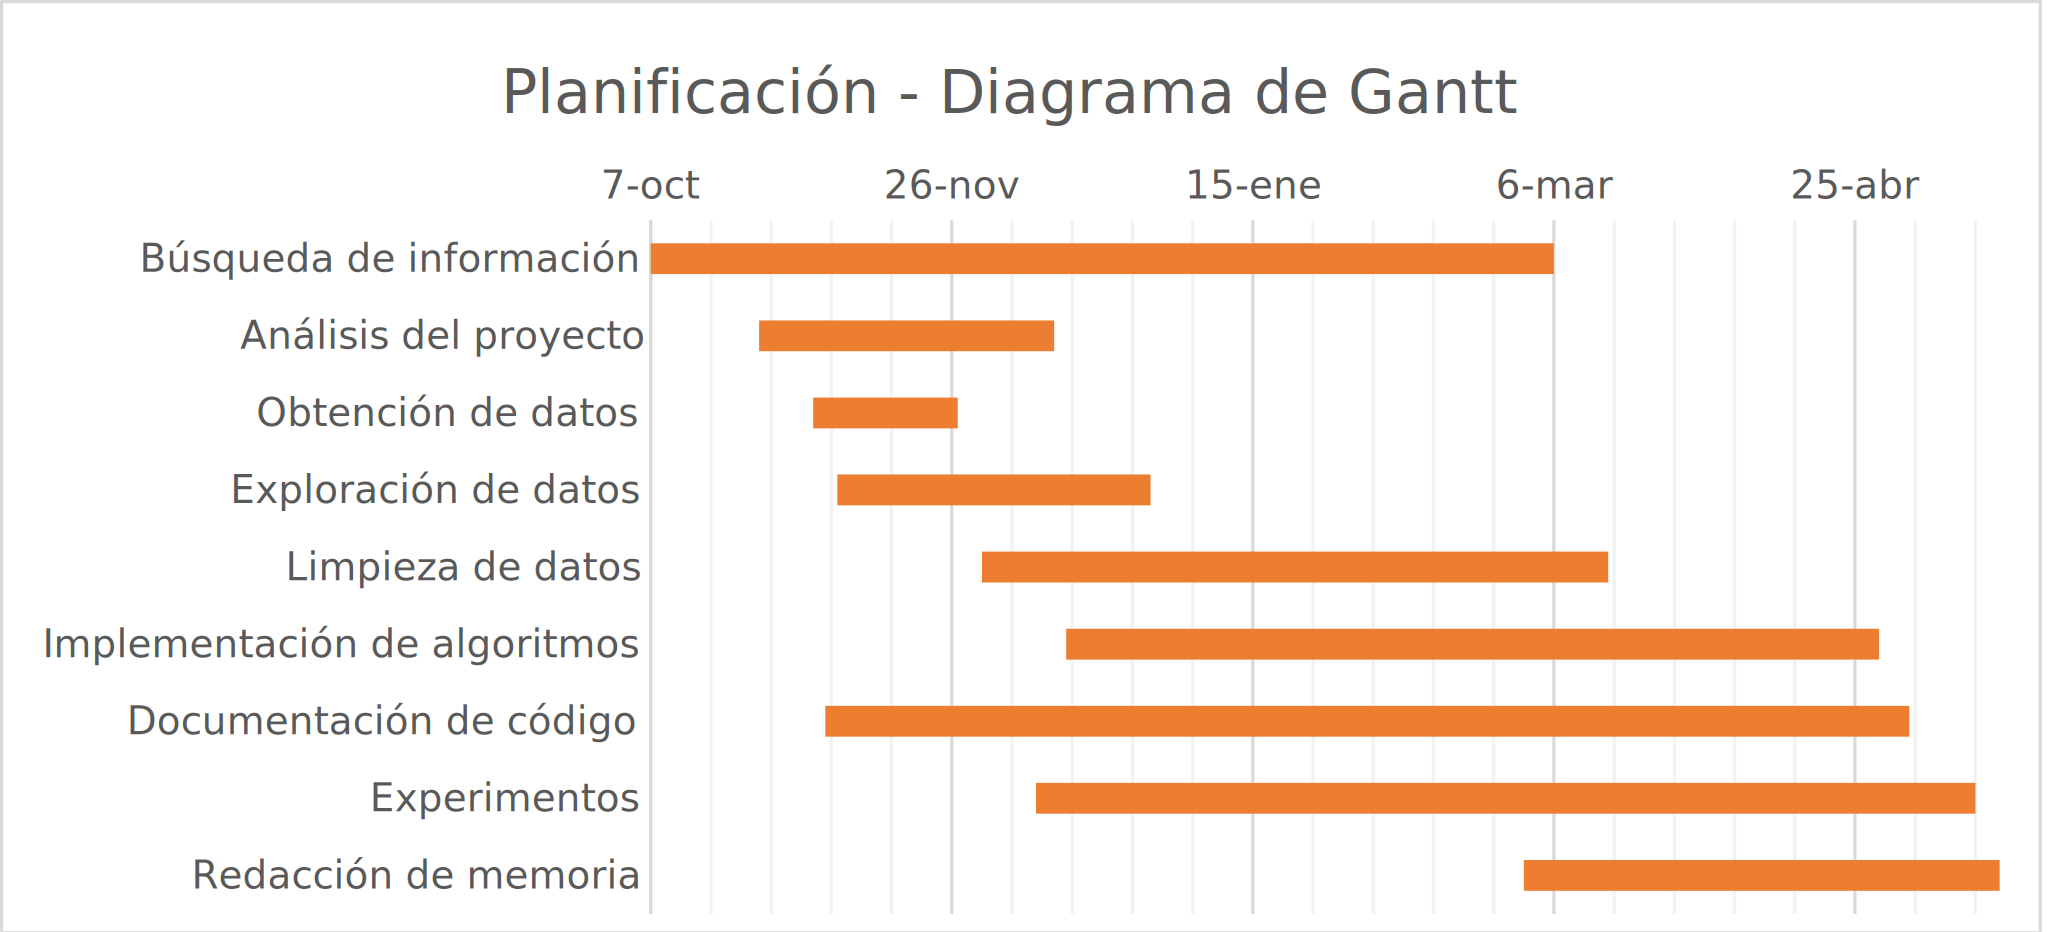
\includegraphics[width=15cm]{archivos/4.Metodologia/GranttImage}
        \caption{Diagrama de Gantt de la planificación del proyecto.}
        \label{GranttImage}
    \end{figure}

    La búsqueda de información incluye la investigación de todo lo referente al proyecto, desde qué es una red neuronal hasta cómo diseñar sus arquitecturas. Por este motivo esta fase es la primera en el desarrollo y ha  sido  un  proceso que se ha prolongado durante casi toda la evolución del trabajo.

    El análisis del proyecto consiste en estudiar la viabilidad del mismo, buscando fuentes de información desde las que poder obtener los datos además de explorarlos. Es una de las fases más críticas en un proyecto \textit{Data Science} ya que si las conclusiones del estudio de viabilidad no son sólidas, se podría cometer el riesgo de empezar un proyecto que no es factible para el cubrir los objetivos.

    La obtención de datos consiste en la búsqueda de repositorios donde encontrar datos que contengan la información requerida para abarcar los objetivos del proyecto, se ha realizado visitando distintos portales de datos abiertos nacionales hasta encontrar un conjunto de datos que encajase con los objetivos, en esta fase también se involucra la exploración inicial de los datos.

    La exploración de datos abarca la fase de análisis de datos, esto se realiza utilizando métodos visuales para entender las características propias del dataset, además de hacer una valoración de la calidad de los mismos. Las primeras etapas de esta fase se complementan con el análisis del proyecto.

    El siguiente paso ha sido la limpieza de datos, gracias a la exploración se comprenden la naturaleza de los datos y se decide qué tecnicas usar para el tratamiento de valores atípicos del conjunto de datos para su posterior transfomación.

    Una de las tareas más importantes en el ciclo de vida de desarrollo Software que garantizan la calidad del producto es la documentación de código. Tiene como fin
    clarificar conceptos y explicar el funcionamiento de los métodos que componen el desarrollo. Es una fase que se prolonga desde el inicio de la codificación en la limpieza de datos hasta poco tiempo después de terminar de implementar los modelos.

    La última fase de este proyecto a nivel funcional de este proyecto ha sido la realización de experimentos, comienza poco antes que la implementación de los modelos y consiste en testar las distintas implementaciones, tanto de limpieza de datos como el funcionamiento de los modelos.

    La última etapa consiste en la redacción de este documento, plasmando toda la información obtenida durante la evolución del proyecto en esta memoria.



\section{Diagrama de flujo}

    En primer lugar se define el flujo de ejecución del proyecto como se muestra en la figura \ref{DataflowImage}, donde se han dividido las etapas del proyecto en seis bloques claramente diferenciados. Cada uno de estos está orientado a una disciplina distinta en proyectos de \textit{Ciencia de Datos} y por lo tanto serán detallados en cada una de las subsecciones posteriores.


    \begin{figure}[H]
        \centering
        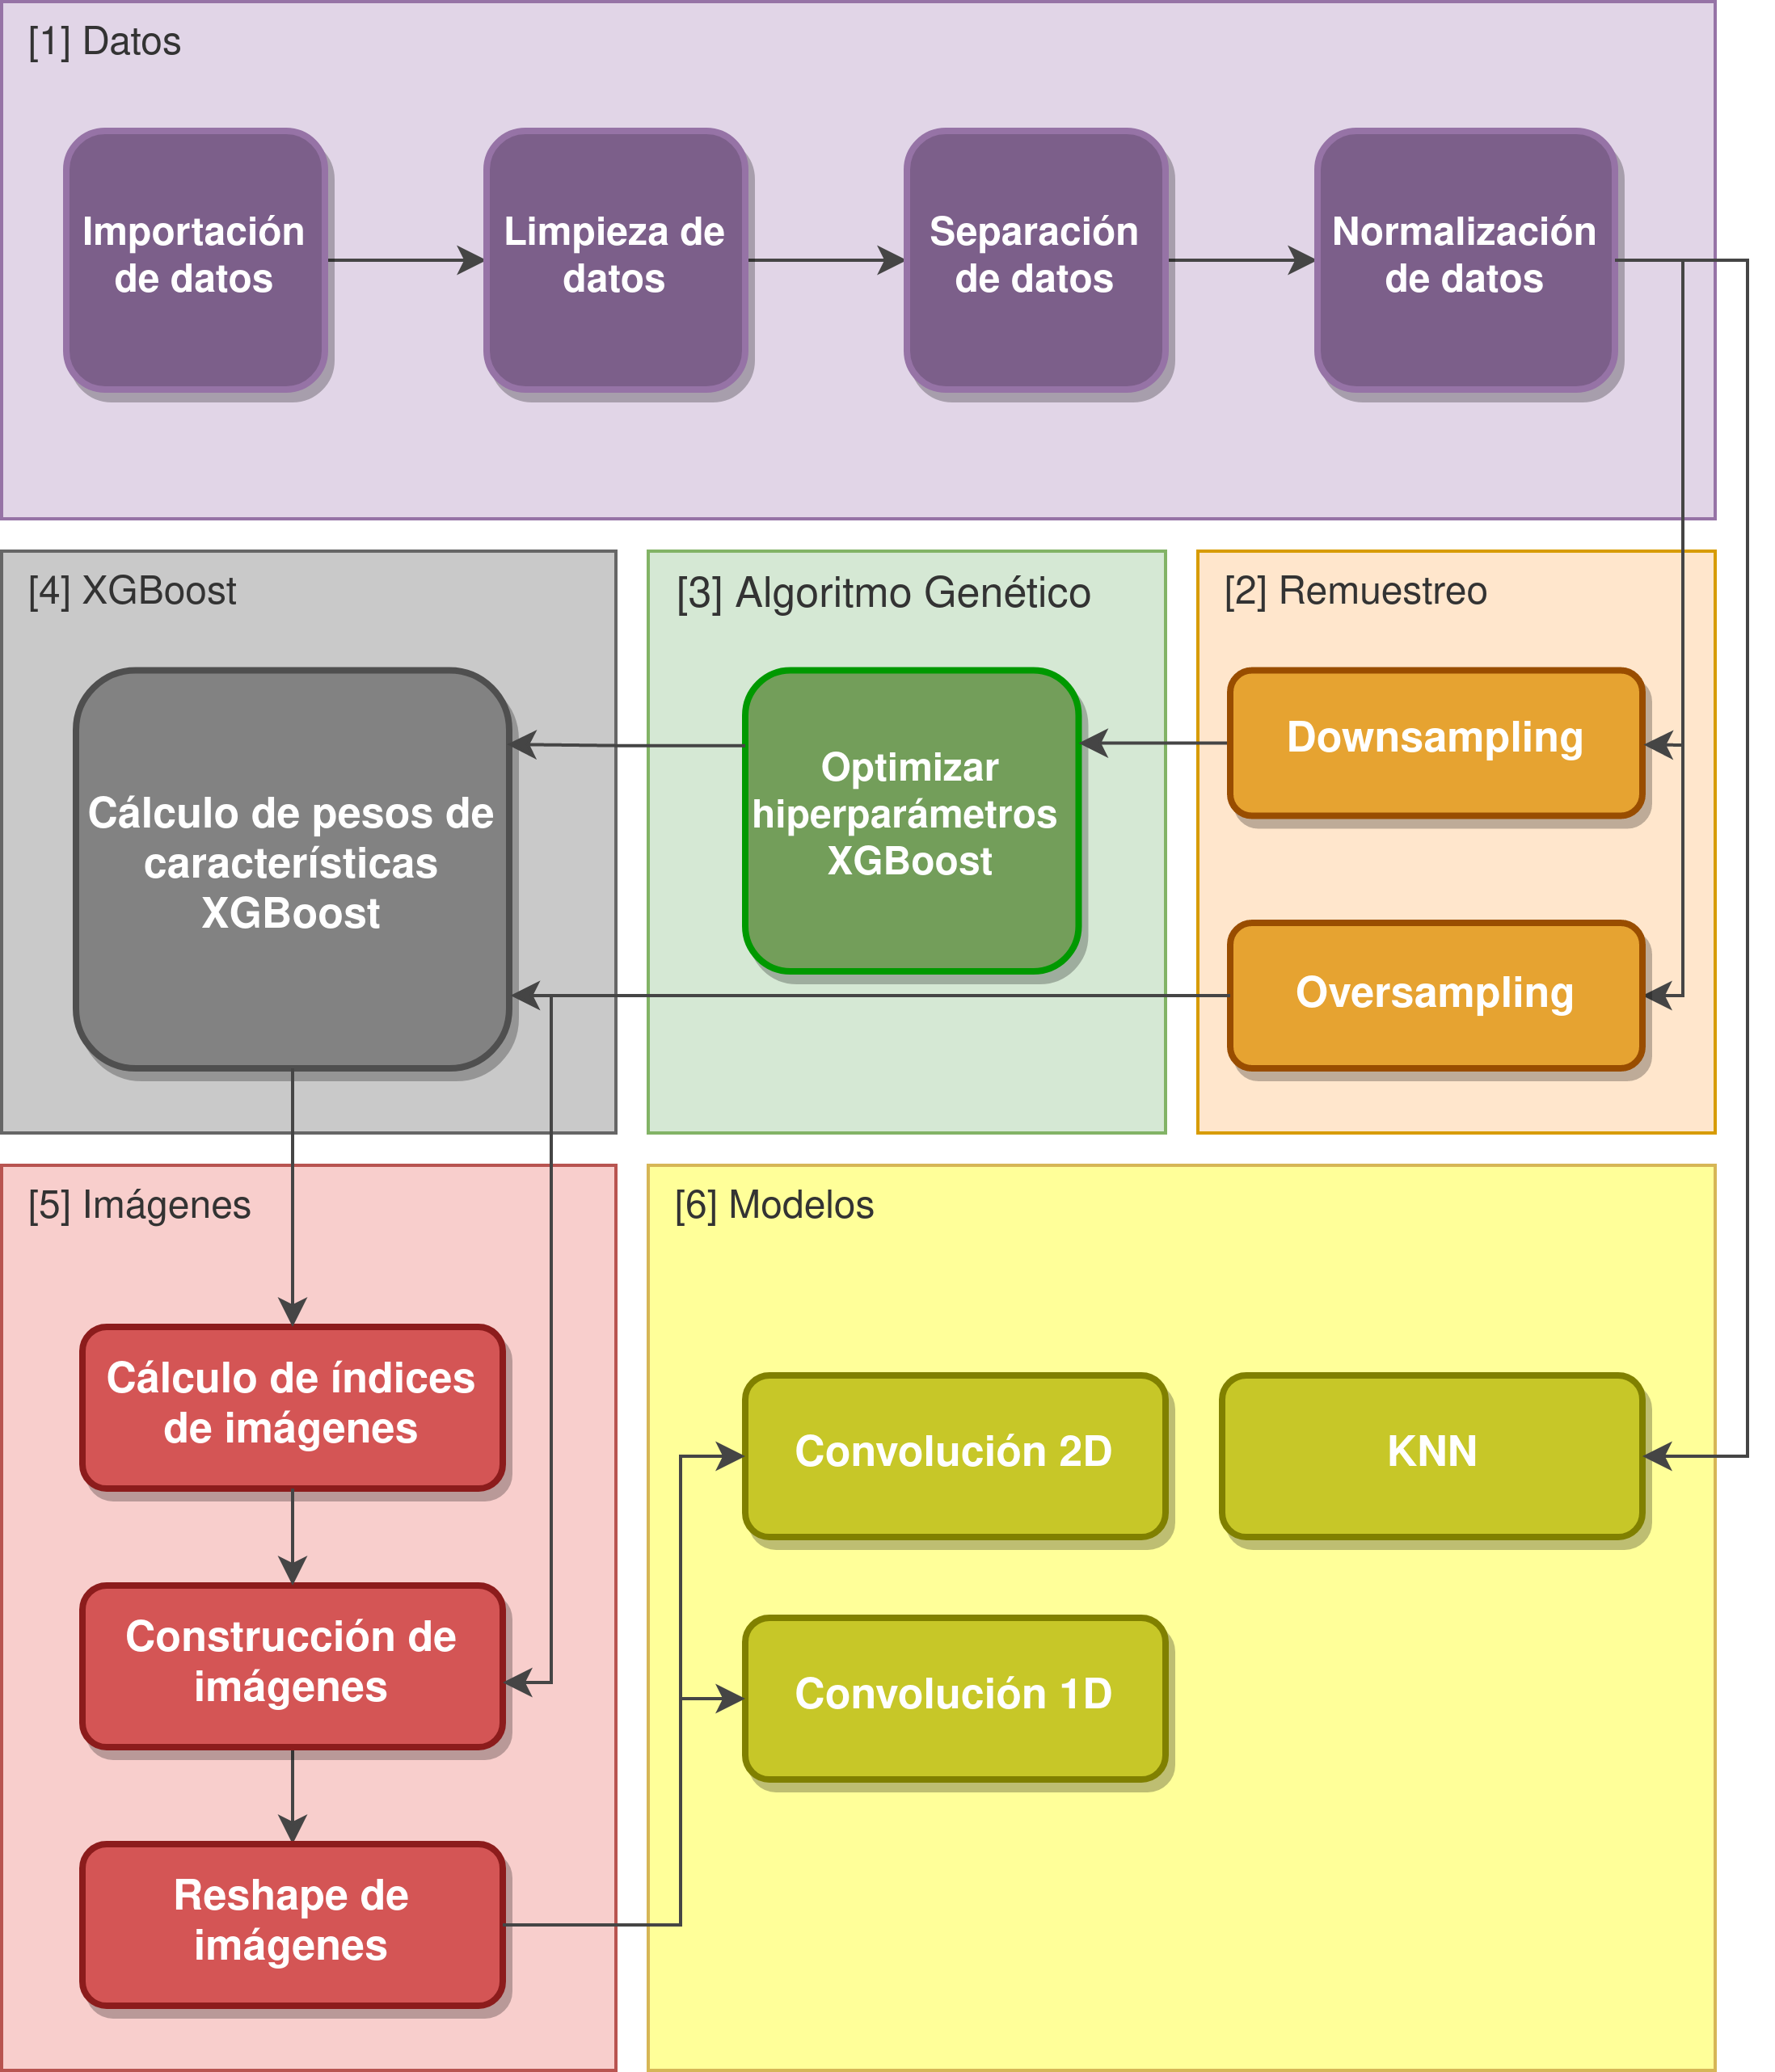
\includegraphics[width=15cm]{archivos/4.Metodologia/DataflowImageESP}
        \caption{Flujo de datos del proceso del proyecto.}
        \label{DataflowImage}
    \end{figure}


\section{Proceso}

    En esta sección describiremos cada uno de los pasos que ha seguido el desarrollo del proyecto, desde la búsqueda inicial de datos hasta la implementación final de los algoritmos:

    \subsection{Datos}


            Como en cualquier proyecto de \textit{Ciencia de Datos} el primer paso contempla la obtención, preparación y estudio de los datos. Este es el proceso en el que más tiempo se invierte en el ciclo de vida de un proyecto, algunos estudios apuntan que alrededor del 80 por ciento del tiempo en un proyecto se destina a esta tarea \cite{LifecycleDataScienceProjectsTimes}, por lo que es extremadamente importante aplicar buenas prácticas a la hora de llevar a cabo esta fase.

            El conjunto de datos con el que se ha trabajado en este proyecto describe accidentes de tráfico de la ciudad de Madrid en un periodo concreto, desde el año 2019 hasta el 2022. Este dataset ha sido obtenido desde \cite{DatasetMadrid}, repositorio donde es posible encontrar distintos datasets relativos a la Comunidad de Madrid.

            El número total de registros en este periodo de tiempo es de 60.966 instancias, cada una de las cuales consta de 17 características que se describirán en la tabla \ref{DescripcionDatosTabla}:

            \renewcommand{\arraystretch}{1.5}
            \begin{table}[H]
                \centering
                \begin{tabular}{|c|L{0.7\textwidth}|}
                    \hline
                    \textbf{Atributo}&\textbf{Descripción}\\
                    \hline
                    \texttt Número de expediente &
                    Identificador del incidente, si varios registros tienen el mismo un número de expediente se consideran como un mismo accidente y cada registro representa cada una de las distintas personas involucradas en él (Conductor, Pasajero o Peatón).\\
                    
                    \hline
                    \texttt Fecha &
                    Día mes y año en el que se ha producido el incidente.\\
                    
                    \hline
                    \texttt Hora &
                    Hora y minuto del día.\\

                    \hline
                    \texttt Localización &
                    Nombre de la calle (si procede).\\

                    \hline
                    \texttt Número &
                    Número de la calle donde ha ocurrido el incidiente (si procede).\\

                    \hline
                    \texttt Distrito &
                    Nombre del distrito de Madrid donde ha ocurrido el incidente.\\

                    \hline
                    \texttt Tipo de accidente &
                    Tipología de accidente, puede ser de diversos tipos (Colisión doble, Colisión múltiple, Alcance, Choque contra obstáculo, Atropello, Vuelco, Caída, Otras causas).\\

                    \hline
                    \texttt Estado meteorológico &
                    Condiciones climatológicas en el momento del incidente (Despejado, Nublado, Lluvia débil, Lluvia intensa, Granizado o Nevando)\\

                    \hline
                    \texttt Tipo de vehículo &
                    Clasificación en función del tipo de vehículos, p.e. motocicleta, turismo, cuadriciclo, etc.\\

                    \hline
                    \texttt Tipo de persona &
                    Rol de la persona involucrada (Conductor, Pasajero o Peatón)\\

                    \hline
                    \texttt Rango de edad &
                    Intervalo de edad la persona implicada.\\

                    \hline
                    \texttt Sexo &
                    Sexo de la persona implicada (Hombre o Mujer).\\

                    \hline
                    \texttt Lesividad &
                    Consecuencias físicas de la persona implicada, si ha necesitado asistencia sanitaria, si ha sido ingresada o si ha sido mortal.\\

                    \hline
                    \texttt Coordenada X &
                    Coordenada X del accidente en formato \textit{UTM}.\\

                    \hline
                    \texttt Coordenada Y &
                    Coordenada Y del accidente en formato \textit{UTM}.\\

                    \hline
                    \texttt Positivo en alcohol &
                    Si la persona implicada ha dado positivo en el control de alcoholemia (S o N).\\

                    \hline
                    \texttt Positivo en drogas &
                    Si la persona implicada ha dado positivo en el control de estupefacientes (S o N).\\

                    \hline
                \end{tabular}
                \caption{Descripción de los datos.}
                \label{DescripcionDatosTabla}

            \end{table}


            La variable respuesta de este proyecto es la lesividad, siguiendo la descripción del conjunto de datos existen una serie de valores asignados a ésta categoría. Cada uno de ellos pertenece al menos a uno de los siguientes casos:

              \begin{itemize}
                    \item Consecuencias leves: comprende desde aquellas personas que no han resultado heridas hasta aquellas que han necesitado ingresar en un centro hospitalario no más de 24 horas, el tipado numérico de estas casuísticas es el siguiente:

                        \begin{itemize}
                            \item 1: Atención en urgencias sin posterior ingreso.
                            \item 2: Ingreso inferior o igual a 24 horas.
                            \item 5: Asistencia sanitaria ambulatoria con posterioridad.
                            \item 7: Asistencia sanitaria sólo en el lugar del accidente.
                            \item 14: Sin asistencia sanitaria.
                        \end{itemize}

                    \item Consecuencias severas: implicados que han requerido un ingreso hospitalario superior a 24 horas, el tipado numérico del conjunto de datos corresponde al siguiente caso:

                        \begin{itemize}
                            \item 3: Ingreso superior a 24 horas.
                        \end{itemize}

                    \item Consecuencias fatales: víctimas mortales dentro del margen de las 24 horas posteriores al accidente, la asignación numérica a este campo es:

                        \begin{itemize}
                            \item 4: Fallecido 24 horas.
                        \end{itemize}

                \end{itemize}


            Se pueden consultar más detalles de las características del dataset descripción del conjunto de datos del portal \textit{Open Data} de Madrid \cite{InfoDatasetMadrid}.


            \begin{enumerate}

                \item Limpieza de datos

                    Una vez importados los datos en el proyecto, es requisito hacer una limpieza de éstos (\textit{Data Cleaning}), eligiendo las características que serán utilizadas como variables explicativas en las predicciones atendiendo además a los valores de las instancias, ya que pueden contener valores nulos, valores atípicos (\textit{outliers}) o contener valores erróneos. Esta problemática requiere de la aplicación de distintas fases de análisis.

                    En el caso del dataset de accidentes de tráfico de este proyecto se han escogido las siguientes características como variables explicativas \textit{hora, distrito, tipo accidente, estado meteorológico, tipo vehiculo, tipo persona, rango edad, sexo, positivo alcohol, positivo drogas, vehiculos implicados, coordenada x utm, coordenada y utm}.


                    Una vez que se han obtenido los predictores con los que trabajarán los modelos, se han eliminado aquellos registros duplicados y aquellos que tuvieran algún valor nulo en alguno de sus predictores. Por lo tanto, las dimensiones finales del conjunto de datos pasarán a ser 12 variables y 54.364 registros con respecto a las 17 características y 60966 filas originales. 

                \item Transformaciones de datos

                    En esta sección detallaremos las transformaciones sobre los datos que han sido necesarias para que los modelos trabajen con un conjunto de datos bien definido y consistente. Gran parte de los modelos de \glsentryshort{ml} necesitan de datos de entrada numéricos para poder comprenderlos, además existe la necesidad de normalizar estos valores para que estén en la misma escala y el entrenamiento sea exitoso, por lo tanto se requiere de una serie de transformacíones que conviertan las variables categóricas a variables numéricas.

                    En primer lugar ha sido necesario transformar las columnas \textit{coordenada x utm} y \textit{coordenada y utm} a números enteros, ya que estas variables eran inicialmente de tipo \textit{String}. Además, se da el caso de que el rango de estas variables es del orden de 7 a 10 dígitos, evitando cualquier formato de decimales estandarizado (utilizando puntos y comas indistintamente en distintas posiciones de los mismos), debido a esto ha sido necesario crear un proceso que analizase cada casuístca y los tradujese a un formato estandarizado.

                    Las columnas \textit{positiva alcohol} y \textit{positiva drogas} se han unido en una nueva columna debido a la cantidad de valores nulos que existía en la segunda variable, por lo que se crea una nueva columna que hace referencia a la intoxicacion etílica o de estupefacientes.
  

                    La variable \textit{localización} ha sido transformada a \textit{tipo de carretera}, con el objetivo de definir un criterio para clasificar el tipo de vía donde se ha producido el incidente, como por ejemplo una carretera, una autovía, glorieta, etc. Al no existir un servicio que ofrezca la tipología de la calle dado el nombre de la vía o las coordenadas UTM, ha sido necesario tratar esta problema desde otro punto de vista mediante expresiones regulares.

                    El término \textit{expresión regular} debe su origen a la teoría de las matemáticas y ciencias de computación, reflejan la propiedad de \textit{regularidad} que caracterizan a las expresiones matemáticas \cite{RegeXBook}. Una expresión regular es un tipo de patrón utilizado para encontrar una combinación de caracteres en una cadena de texto. Para clasificar el tipo de carreteras en este proyecto se han diseñado una serie de expresiones regulares que coinciden con ciertos criterios respecto a los valores de la variable \textit{localizacion} con el fin de distinguir distintos tipos de vía.


                    \textbf{NOTA: Ponemos una tabla con todas las RegEx que se han utilizado? Es sin duda la peor parte y menos científica del proyecto, y es lo único que no me gustaría mostrar, aunque ha llevado mucho tiempo me daría un poco de vergüenza poner esto en un proyecto de Ciencia de datos la verdad}


                    Las tipologías de clases de carreteras son \textit{Parking, Aeropuerto, Cuesta, Paseo, Parque, Túnel, Polígono, Camino, Glorieta, Puerta, Puente, Plaza, Bulevar, Travesía, Calzada, Carretera, Avenida, Autovía} y \textit{Calle}


                    No obstante, la aplicación de las expresiones regulares generalmente no son una solución empírica a un problema, ya que hay casos que se pueden ser no contemplados al diseñar estos patrones manualmente, y en el caso de este proyecto su aplicación conlleva una serie de inconvenientes. Debido a las necesidades del problema están diseñadas jerárquicamente, de tal forma que aquellos valores de la variable \textit{localizacion} que coincidan con el primer patrón definido de la expresión regular serán asignados a esta categoría. Esto supone un impedimento a tener en cuenta, ya que muchos de los accidentes se producen en intersecciones, carriles de aceleración que conectan dos vías, vías cuyo nombre contiene el tipo de otra vía, etc. Si se da el caso de que haya algún patrón que no se ha definido como expresión regular, provocará que estas localizaciones se asignen con respecto al primer patrón definido encontrado, llegando a clasificar erróneamente el tipo de vía. Como consecuencia, el orden de la definición de las expresiones es un punto crítico porque se busca maximizar la clasificación de aquellos tipos de vía con menor número de apariciones, como es el caso de parking o aeropuerto, mientras se busca minimizar el error en la clasificación.


                    Para solucionar esto herramientas como Open Refine \cite{OpenRefine} que utilizan técnicas de clustering nominal para detectar semejanzas entre nombres podría ser una solución.

                    Por otra parte hay que tratar aquellos valores que no hayan coincidido con los patrones definidos (TODO: poner el número), sin embargo, al ser una cantidad de registros se han podido revisar manualmente coincidiendo todas con nombres de calles al que no se les ha asignado la palabra \textit{"calle"}.


                    En la variable \textit{hora}, al ser un campo continuo ha sido necesario discretizarla según intervalos, distinguiendo entre noche y día en función de la hora en la que se ha producido el incidente.


                    En la tabla \ref{TransformacionDatosTabla} se define el resto de codificaciones aplicadas sobre el resto de variables del modelo para transformar estos campos a formato numérico.

                    \def\arraystretch{1.2}%
                    \begin{longtable}{|c|L{0.7\textwidth}|}\\

                        \hline
                        \textbf{Característica} & \textbf{Tipado}\\

                        \hline
                        \multirow{3}{*}{Lesividad}              & 0: Accidentes leves (\textit{1, 2, 5, 6, 7, 14}).\\
                                                                & 1: Accidentes severos (\textit{3}).\\
                                                                & 2: Accidentes fatales (\textit{4}).\\

                        \hline
                        \multirow{2}{*}{Hora}                   & 1: Noche (\textit{6 PM - 6 AM}).\\
                                                                & 2: Día (\textit{6 AM - 6 PM}).\\
                        \hline
                        \multirow{1}{*}{Distrito}               & Numeración en función de orden de aparición.\\

                        \hline
                        \multirow{2}{*}{Tipo Accidente}         & 1: Colisión fronto-lateral. \\
                                                                & 2: Alcance.\\
                                                                & 3: Colisión lateral.\\
                                                                & 4: Choque contra obstáculo fijo.\\
                                                                & 5: Colisión múltiple.\\
                                                                & 6: Caída.\\
                                                                & 7: Atropello a persona.\\
                                                                & 8: Colisión frontal.\\
                                                                & 9: Otro.\\
                                                                & 10: Solo salida de la vía.\\
                                                                & 11: Vuelco.\\
                                                                & 12: Atropello a animal.\\
                                                                & 13: Despeñamiento.\\
                        \hline
                        \multirow{7}{*}{Estado Meteorológico}   & 1: Despejado.\\
                                                                & 2: Nublado.\\
                                                                & 3: Lluvia débil.\\
                                                                & 4: Lluvia intensa.\\
                                                                & 5: Granizando.\\
                                                                & 6: Nevando.\\
                                                                & 7: Se desconoce.\\
                        \hline
                        \multirow{1}{*}{Tipo Vehículo}          & Numeración en función de orden de aparición.\\

                        \hline
                        \multirow{3}{*}{Tipo Persona}           & 1: Conductor.\\
                                                                & 2: Pasajero.\\
                                                                & 3: Peatón.\\
                        \hline
                        \multirow{5}{*}{Rango Edad}             & 1: Menores de 18 años.\\
                                                                & 2: De 18 a 25 años.\\
                                                                & 3: De 25 a 65 años.\\
                                                                & 4: Mayores de 65 años.\\
                                                                & 5: Edad desconocida.\\
                        \hline
                        \multirow{3}{*}{Sexo}                   & 1: Hombre.\\
                                                                & 2: Mujer.\\
                                                                & 3: Desconocido.\\
                        \hline
                        \multirow{2}{*}{Positivo}               & 1: Sí.\\
                                                                & 2: No.\\
                        \hline

                    \caption{Transformaciones aplicadas a los datos.}
                    \label{TransformacionDatosTabla}\\
                    \end{longtable}


                \item Análisis de datos

                    Una de las fases más importantes antes de comenzar el modelado en cualquier proyecto \textit{Data Science} es el análisis de datos. Este proceso tiene como objetivo la descripción de los datos, identificación de \textit{outliers}, valores erróneos y tendencias que se puedan dar en ellos.\\

                    Comenzaremos analizando los datos que correspondan a cada una de las tres posibles clases (leves, severos y fatales) realizando un histograma \ref{OriginalDataHistogramImage}. Como podemos observar, nos encontramos ante un dataset claramente desbalanceado con respecto a la variable respuesta, contando con 53.009 accidentes leves, 1.271 severos y 84 fatales.\\

                    Un conjunto de datos desbalanceado se define como aquel que contiene un número de instancias mucho mayor de determinadas clases con respecto al resto \cite{WhyImbalancedDataIsAProblem}. Esto se convierte en un problema para los modelos de clasificación ya que estos modelos tenderán a predecir las muestras como aquellas que pertenecen a las mayoritarias sobre el conjunto de test debido a que las reglas de classificación de las clases menos numerosas tienden a ser ignoradas.

                    El desbalanceo de datos es un problema ampliamente estudiado a lo largo de los años y existen numerosos métodos orientados a solventarlo mediante distintas técnicas de muestreo \cite{ImbalancedDataReview}, por lo que será necesario aplicar distintas técnicas sobre el conjunto de datos.


                    \begin{figure}[H]
                        \centering
                        \includesvg[scale=0.3]{archivos/4.Metodologia/Datos/Analisis/OriginalDataHistogram}
                        \caption{Histograma de clases de accidente en el conjunto de datos original.}
                        \label{OriginalDataHistogramImage}
                     \end{figure}


                    En la figura \ref{CorrelationMatrixImage} podemos observar la matriz de correlación de las variables explicativas del conjunto de datos del proyecto. Esta matriz muestra las relaciones existentes entre las variables indicando el grado de correlación entre ellas. Estos valores están acotados entre [-1, 1] en base al coeficiente de correlación de \textit{Pearson} \cite{PearsonCoefficientCorrelationMatrix}, que indica la relación entre pares de campos, de tal forma es posible saber tanto el grado como la proporcionalidad de esta variación.

                    Analizando la matriz se puede comprobar que las únicas variables que están medianamente correlacionadas son \textit{coordenada x utm} y \textit{distrito}, con una correlación positiva de 0.44, sin embargo no es un valor tan alto como para eliminar alguna de las dos las características.

                    \begin{figure}[H]
                        \centering
                        \includesvg[scale=0.3]{archivos/4.Metodologia/Datos/Analisis/CorrelationMatrix}
                        \caption{Matriz de correlación para los predictores escogidos del dataset.}
                        \label{CorrelationMatrixImage}
                     \end{figure}


                \item Normalización de datos

                    La normalización de datos es un proceso necesario a la hora de obtener buenos resultados en los modelos predictivos de \glsentryshort{ml}. Cuando un modelo es entrenado, es bastante probable existan características representadas en distintas escalas. En consecuencia, las características que contengan un rango de valores numérico más alto, ya sea por la naturaleza de la variable o porque se encuentren en otro rango, dominarán a aquellas características que contengan un rango menor, influenciando negativamente a los modelos \glsentryshort{ml}, que normalmente son muy sensibles a la desnormalización de datos, como por ejemplo las \glsentryshort{cnn} o \glsentryshort{knn} \cite{NormalizationSensitiveModels}.\\

                    El proceso de normalización tiene como objetivo minimizar el \textit{bias} de aquellas características cuya contribución sea mayor a la hora de encontrar patrones entre los datos. Existen distintas técnicas de normalización como por ejemplo \glsentryfull{mc}, \glsentryfull{vss} o \glsentryfull{mmn} entre otras \cite{DataNormalizationInvestigation}.\\


                    En este proyecto se ha utilizado la normalización \glsentryfull{zsn} debido a las propiedades que ofrece, \glsentryshort{zsn} que utiliza la media y la desviación típica para reescalar los datos de tal forma que la distribución de ellos esté definida por una media de cero y una desviación típica unitaria, consiguiendo representaciones de acuerdo a una distribución normal.\\

                    Los resultados obtenidos después de aplicar esta técnica se pueden interpretar como la distancia de cada valor con respecto a la media.

                   \begin{center}
                        $x^* = \frac{x - u}{\sigma}$
                    \end{center}


                    Donde $x^*$ es una muestra de una característica de los datos, $u$ es la media total de dicha característica y $\sigma$ es la desviación típica total de los valores de la característica.


                \item Separación de datos

                    La siguiente fase en cualquier modelo de \glsentryshort{ml} es la separación de datos (\textit{split}). Esta fase consiste en dividir el conjunto total de registros en al menos dos subconjuntos, uno de entrenamiento y otro de test. El modelo se entrenará en base al conjunto de entrenamiento y se evaluará con el de test, los resultados sobre este conjunto permitirán comparar los modelos en base a las predicciones sobre las muestras que nunca han visto.\\


                    Comúnmente la proporción de datos de entrenamiento y test está establecida en \textit{0.8} y \textit{0.2} respectivamente, en la figura \ref{DataSplitImage} se muestra una representación visual de esta división.


                    \begin{figure}[h]
                        \centering
                        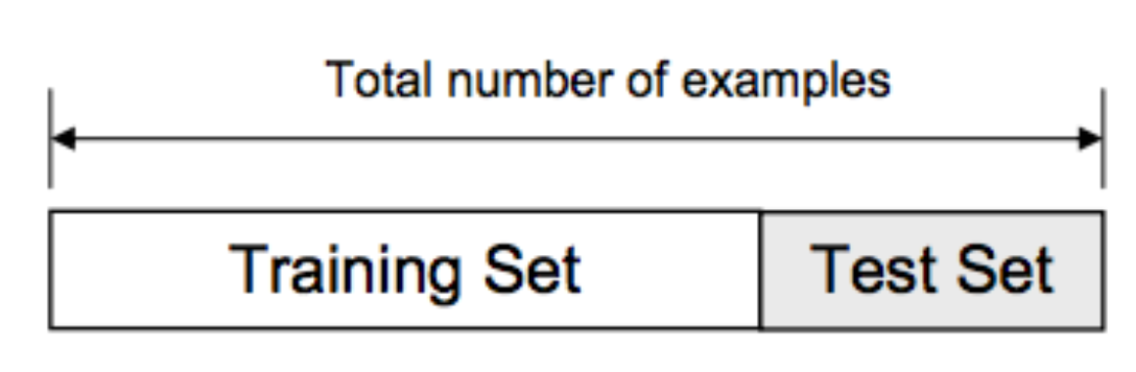
\includegraphics[width=7cm]{archivos/4.Metodologia/Datos/Separacion/DataSplit}
                        \caption{https://towardsdatascience.com/train-test-split-and-cross-validation-in-python-80b61beca4b6. División de un conjunto de datos en datos de entrenamiento y test.}
                        \label{DataSplitImage}
                     \end{figure}

            \end{enumerate}



        \subsection{Remuestreo}


            Son técnicas permiten operar sobre el conjunto de datos para balancearlo, con el objetivo de que el modelo no se vea muy afectado debido a la diferencia de las clases mayoritarias respecto a las minoritarias. Estas técnicas de forma general se aplican únicamente al conjunto de entrenamiento, ya que la intención  es influir sobre el aprendizaje del modelo para aumentar el rendimiento de las predicciones sobre el conjunto de test, si aplicásemos remuestreo sobre este último conjunto estaríamos falseando los resultados de las predicciones.


            En este proyecto se han hecho uso de las siguientes técnicas de remuestreo:

            
            \begin{enumerate}



                \item Downsampling: tiene como objetivo balancear el conjunto de datos para que todas las clases tengan el mismo número de muestras igualando el número de muestras de las clases mayoritarias a aquellas clases que contienen menos muestras, descartando aquellas que sobrepasen este límite \cite{Downsampling}. \textbf{NOTA: Aún no se sabe si se va a aplicar Downsampling o no, sigo con los experimentos, de momento lo dejaré así a la espera de ver más resultados, queda pendiente para revisión}
                

                \item Generación de datos sintéticos: técnica que permite generar datos artificiales en base a los límites que separan unas clases de otras. Se ha hecho uso de la tećnica \glsentryfull{smoteii} \cite{SMOTEII}. Esta técnica selecciona los vecinos más cercanos de la misma clase y genera nuevas muestras en base al espacio entre la clase minoritaria y sus vecinos más cercanos.\\

                \glsentryshort{smoteii} ha sido utilizado para generar más muestras artificiales de los accidentes pertenecientes a las clases minoritarias (\textit{severos} y \textit{graves}). Este nuevo conjunto de datos servirá como entrenamiento para los modelos, evitando que tiendan al sobreajuste. En la figura \ref{SMOTEIIDataHistogramImage} se aprecia el histograma tras haber aplicado \glsentryshort{smoteii}, contando ahora con 42508 muestras de cada una de las clases de accidentes.

                \begin{figure}[H]
                    \centering
                    \includesvg[scale=0.3]{archivos/4.Metodologia/Datos/Analisis/SMOTEIIDataHistogram}
                    \caption{Histograma de clases de accidente del conjunto de entrenamiento tras aplicar SMOTE-II.}
                    \label{SMOTEIIDataHistogramImage}
                 \end{figure}

            \end{enumerate}


            Una vez aplicadas las técnicas de remuestreo, es útil observar cuál es la representación espacial de los datos sintéticos generados por \glsentryshort{smoteii} en deferencia a los datos originales mediante el método \glsentryfull{tsne} \cite{TSNEPaper}. \glsentryshort{tsne} es un algoritmo que permite visualizar las proyecciones de datos multidimensionales en espacios bidimensionales o tridimensionales. Este modelo debe su origen a su antecesor \glsentryfull{sne}, siendo una versión optmizada de éste.

            Mientras que \glsentryshort{sne} proyecta los datos conviritiendo las distancias Euclídeas entre las muestras a probabilidades condicionales sean similares entre sí siguiendo probabilidades normales, el \glsentryshort{tsne} modifica la función de coste para proyectarlos mediante una distribución t-Student, permitiendo además trabajar con gradientes simplificados.


            En la figura \ref{TSNEImages} se muestran las proyecciones de \glsentryshort{tsne} (tanto la representación bidimensional como la tridimensional) sobre el conjunto de datos de entrenamiento original y aquellos que han sido generados artificialmente por \glsentryshort{smoteii}.

            El \glsentryshort{tsne} de 2D aplicado sobre los datos generados por \glsentryshort{smoteii} \ref{TSNEImages:Train2D} nos permite observar cómo se han generado las muestras con respecto a los datos originales \ref{TSNEImages:Clean2D} en una proyección bidimensional. Se aprecia cómo se han producido las nuevas muestras de los accidentes graves (azul) calculando la cercanía de los puntos en base a las fronteras de división. \textbf{Nota: Realmente yo no veo nada}.


            \begin{figure}
                \centering
                \begin{subfigure}[b]{0.4\textwidth}
                    \centering
                    \includesvg[scale=0.4]{archivos/4.Metodologia/Datos/Resampling/TSNE/2d_tsne_clean}
                    \caption{TSNE de 2 componentes aplicado a los datos originales.}
                    \label{TSNEImages:Clean2D}
                \end{subfigure}
                % Añadir el espacio deseado, si se deja la linea en blanco la siguiente subfigura ira en una nueva linea
                \begin{subfigure}[b]{0.4\textwidth}
                    \centering
                    \includesvg[scale=0.4]{archivos/4.Metodologia/Datos/Resampling/TSNE/2d_tsne_train}
                    \caption{TSNE de 2 componentes aplicado a los datos generados por SMOTE-II.}
                    \label{TSNEImages:Train2D}

                \end{subfigure}
                \begin{subfigure}[b]{0.4\textwidth}
                    \centering
                    \includesvg[scale=0.4]{archivos/4.Metodologia/Datos/Resampling/TSNE/3d_tsne_clean}
                    \caption{TSNE de 3 componentes aplicado a los datos originales.}
                    \label{TSNEImages:Clean3D}
                \end{subfigure}
                \begin{subfigure}[b]{0.4\textwidth}
                    \centering
                    \includesvg[scale=0.4]{archivos/4.Metodologia/Datos/Resampling/TSNE/3d_tsne_train}
                    \caption{TSNE de 3 componentes aplicado a los datos generados por SMOTE-II.}
                    \label{TSNEImages:Train3D}
                \end{subfigure}
                \caption{TSNE de 2 y 3 componentes aplicado a los datos originales y a los generados sintéticamente (\glsentryshort{smoteii}).}
                \label{TSNEImages}
             \end{figure}



    \subsection{Algoritmo Genético}


        Para un ideal entrenamiento de un modelo predictivo es conveniente optimizar los hiperparámetros con los que el modelo será entrenado, en este proyecto se aplicarán los algoritmos genéticos para optimizar hiperparámetros del algoritmo \glsentryshort{xgboost}.\\

        Para ello se ha hecho uso de algoritmos genéticos \cite{GAXGBoostCode}, donde cada individuo perteneciente a la población de una generación está formado por una configuración de hiperparámetros específica, de tal forma que a lo largo de las iteraciones los individuos evolucionarán mediante el cruce y la mutación para dar lugar a nuevas configuraciones de hiperparámetros optimizadas \cite{GAXGBoostPaper}.

        Debido al coste computacional que tendría optimizar todos los parámetros por la magnitud del espacio de búsqueda y al no ser necesario tener en cuenta todos ellos, se ha seleccionado un subcojunto de aquellos que más influencia tienen en el entrenamiento del modelo. Los hiperparámetros de los que consta cada individuo de la población son:

        \begin{enumerate}

            \item Profundidad máxima: es la máxima altura que puede tomar el árbol. Si el árbol de decisión alcanza demasiada profundidad tenderá al \textit{overfitting} ya que aprenderá relaciones complejas entre los datos que pueden deberse a ruido en los datos de entrenamiento.

            \item Peso mínimo de los hijos: es el mínimo peso que se establece a la hora de crear un nuevo nodo en el árbol. Cuando se entrena un árbol de decisión éste genera nuevos nodos en base a máxima separabilidad de los datos de entrenamiento en cada nivel. Con el límite de peso de los hijos establecemos un umbral mínimo de muestras que deben pertenecer a un nodo para realizar la separación. Un valor bajo en este parámetro permitirá crear nodos con menos muestras y por lo tanto el modelo tenderá al \textit{overfitting}.

            \item ETA: tamaño de paso utilizado para aplicar descenso por gradiente para minimizar la pérdida de los árboles anteriores.

        \end{enumerate}

        La inicialización y mutación de los valores de los individuos viene dada por una limitación mínima y máxima que pueden, ya que, si no se contemplase, los hiperparámetros podrían tomar valores extremos, reduciendo así el rendimiento de entrenamiento y el de las predicciones. Por lo tanto los individuos variarán sus parámetros tomando un valor aleatorio dentro de estos rangos definidos.  Los parámetros de las nuevas soluciones mutarán dentro de unos límites específicos para cada parámetro establecidos como máximos y mínimos para que no tomen valores extremos. La tabla \cite{InitAndMutationLimitsHyperparamsTable} muestra los límites de los hiperparámetros.

        \begin{table}[H]
            \centering
                \begin{tabular}{ |c|c|c| } 
                \hline
                \textbf{Hiperparámetro} & \textbf{Inicialización} & \textbf{Mutación}\\
                \hline
                    Profundidad Máxima & [1, 25] & [-6, 6]\\ 
                    Peso mínimo de los hijos & [0.01, 20.0] & [-7, 7] \\ 
                    ETA & [0.01, 1] &  [-0.3, 0.3] \\ 
                \hline

                \end{tabular}

            \caption{Límites de inicialización y mutación de los hiperparámetros de los individuos.}
            \label{InitAndMutationLimitsHyperparamsTable}
        \end{table}

        Una vez inicializados aleatoriamente los TODO:X individuos especificados en la población, éstos se evaluarán instanciando TODO:X modelos \glsentryshort{xgboost} con los valores de cada individuo en la población. El conjunto de datos sobre el que entrenará cada instancia \glsentryshort{xgboost} será el conjunto de entrenamiento TODO:XX. La función \textit{fitness} que evaluará cada individuo será la métrica TODO:F1-X aplicada sobre el conjunto de test obtenido en el proceso de separación de datos.

        \textbf{TODO: No se redactará más hasta tener claro cuál es la mejor forma de entrenar el \glsentryshort{xgboost} (función de validación y datos de entrenamiento)}





        %SE HACE CON EL CONJUNTO DE ENTRENAMIENTO DOWNSAMPLED
        %SE TESTA CON VALIDACION

    \subsection{XGBoost}


        \textbf{TODO: Decir si se entrena con downsampled o smote-ii en función de los experimentos cuando acabemos}\\

        Una vez se han optimizados los hiperparámetros del \glsentryshort{xgboost}, se entrena un nuevo modelo con los pq4m354ow calculados sobre el conjunto de entrenamiento remuestreado. Con este nuevo modelo \glsentryshort{xgboost} entrenado se obtiene la importancia de cada clase mediante la ponderación de sus pesos. \cite{XGBoostFeatureWeightsMeaning}. Estos pesos son calculados por \glsentryshort{xgboost}, e indican el grado de importancia que ha tenido cada característica del conjunto de datos a la hora de entrenar el árbol, por lo tanto, aquellas caracerísticas a las que se les asigne más peso habrán sido aquellas que han jugado un papel clave en las decisiones de los árboles.

        Los pesos son asignados para cada característica del conjunto de datos con el que ha sido entrenado \glsentryshort{xgboost} de tal forma que permite realizar un análisis comparativo de los atributos y saber qué predictores son más importantes.


    \subsection{Imágenes}


        Las \glsentryshort{cnn} aprenden patrones sobre la entrada de datos como imágenes, esto implica que éstas estén construidas de tal forma que se maximice la representación de la información, es decir, es necesario aplicar técnicas que posicionen cada característica en un pixel de la matriz maximizando la representación de los accidentes (TODO: \textbf{relamente no entiendo muy bien la motivación que ha seguido la gente de TASPCNN a la hora de construir las imágenes, falta entender por qué lo hacen así, no lo he encontrado en el paper.})

        Por lo tanto, una vez se tienen los datos normalizados y muestreados, el siguiente paso será transferir cada una de las muestras tabulares de los accidentes a una imagen en escala de grises, donde a cada característica se le asignará una posición de la matriz (\textit{5 x 5}), de tal forma que éstas sean la entrada a las \textit{CNN}.

        Para este objetivo se aplicará el algoritmo FV2GI propuesto en el artículo \cite{TASPCNN}, que asigna las características de una muestra en representación tabular en función de la importancia que éstas presenten en una jerarquía.

        Tal y como se propone en \cite{JerarquiaImagenes} las características que provocan un accidente de tráfico pueden englobarse en una serie de elementos o categorías principales, concretamente: \textit{características del conductor, el estado de la carretera, características propias del vehículo y condiciones del ambiente}. Por este motivo se realizará una asignación de cada característica del dataset en una de estas categorías, se muestra en la tabla \ref{JerarquiaCaracteristicasTabla} las asignaciones de las variables explicativas del conjunto de datos en función de esta jerarquía.


        \begin{table}[H]
          \centering
          \begin{tabular}{ |c|c| }
               \hline
               \textbf{Categoría} & \textbf{Variable}\\

               \hline
               \multirow{4}{*}{Accidente}            & Coordenada X.\\
                                                     & Coordenada Y.\\
                                                     & Hora.\\
                                                     & Vehículos implicados.\\
                                                     & Tipo de accidente.\\

               \hline
               \multirow{1}{*}{Ambiente}             & Estado meteorológico.\\

               \hline
               \multirow{2}{*}{Carretera}            & Tipo Carretera.\\
                                                     & Distrito.\\

               \hline
               \multirow{4}{*}{Conductor}            & Tipo Persona.\\
                                                     & Sexo.\\
                                                     & Rango Edad.\\
                                                     & Positivo.\\

               \hline
          \end{tabular}
          \caption{Transformaciones aplicadas a los datos.}
          \label{JerarquiaCaracteristicasTabla}
        \end{table}



        Una vez definida la jerarquía de características y los pesos asociados a cada una de ellas gracias al algoritmo \glsentryshort{xgboost}, se construyen las imágenes de acuerdo al criterio \textit{FV2GI}. Este proceso consta de los siguientes pasos:

        \begin{enumerate}

            \item Generación de \textit{n} imágenes inicializadas a 0, donde \textit{n} es el número de muestras tabulares en el dataset.
            \item Asignación de una fila a cada padre en función de su peso.
            \item Asignacíón de la la posición de cada característica hija en función de su peso dentro de la fila de su padre.
        
        \end{enumerate}

        Se deben tomar las siguientes consideraciones a la hora de aplicar \textit{FV2GI}:

        \begin{enumerate}

            \item La importancia de un padre viene dada por ĺa suma de los pesos de las características hijas, en la tabla \ref{PesosFinalesCaracteristicas} se observa el cálculo de cada característica para las categorías principales.

            \item La asignación de las filas de los padres se realiza de forma intercalada en función de su peso. Aquel padre que más importancia tenga irá posicionado en la fila central de la matriz, el segundo padre irá posicionado por encima de éste y el tercero por debajo y así sucesivamente, de tal forma que se irá creando una estructura en la que dichos padres se interpolan entre las filas en función de su peso.

            \item Una vez se han asignado las categorías padre a las filas se realiza el mismo procedimiento con las características hijas a nivel de columna. Estas características se asignarán en una posición dentro de la fila de su categoría padre, donde aquella que más importancia tenga irá posicionada en el centro, la segunda irá posicionada a su izquierda, la tercera a la derecha y así sucesivamente.
        \end{enumerate}

        \textbf{Nota: No estoy contento con la explicación, creo que estaría bien meter una fórmula matemática o pseudocódigo y cambiar la redacción}

        Como resultado de este proceso se obtienen las imágenes con un único canal gris \ref{SampledImagesExampleImage}, que serán la entrada de las \glsentryshort{cnn} en forma de representaciones matriciales.

        \begin{figure}[H]
            \centering
            \includesvg[scale=0.5]{archivos/4.Metodologia/Imagenes/GrayImages/madrid_image_example_0}
            \includesvg[scale=0.5]{archivos/4.Metodologia/Imagenes/GrayImages/madrid_image_example_1}
            \includesvg[scale=0.5]{archivos/4.Metodologia/Imagenes/GrayImages/madrid_image_example_2}

            \caption{Representación de las muestras de accidentes en forma de matriz de grises.}
            \label{SampledImagesExampleImage}
        \end{figure}

    \subsection{Modelos}


        En esta sección analizaremos los modelos utilizados en este proyecto con el objetivo de realizar un estudio comparativo entre las arquitecturas.


        \begin{enumerate}

            \item KNN

                El método \glsentryshort{knn} servirá como referencia para testar el rendimiento del resto de modelos. Al ser un método que se aplica sobre un conjunto de datos tabular original, no hará uso de las imágenes generadas.

                Es necesario optimizar los parámetros de este algoritmo para conseguir un buen rendimiento, por lo que aplicaremos la técnica \textit{Grid Search} \cite{GridSearchSklearnLibrary}. Esta técnica permite la optimización de los valores de los hiperparámetros mediante una búsqueda exhaustiva en un espacio de búsqueda definido por el usuario, probando distintas combinaciones hasta cubrirlo por completo. 

                \glsentryshort{knn} construirá el espacio de proyecciones mediante los datos de entrenamineto remuestreados por \glsentryshort{xgboost}, y clasificará las muestras del conjunto de test en base a la cercanía de los vecinos proyectados del conjunto de entrenamiento.


            \item CNN

                Una vez definidos los pasos que sigue el entrenamiento de una \textit{NN} y las características propias de las \textit{CNNs}, podemos analizar las arquitecturas de las \textit{CNNs} implementadas que se han aplicado en este proyecto. Cabe mencionar que el funcionamiento de ambas \textit{CNNs} únicamente difiere en el tamaño del \textit{kernel} (unidimensionales o bidimensionales según sea el caso correspondiente) y la forma en la que éste se desplaza debido a su dimensionalidad, por lo tanto detallaremos ambas arquitecturas de la misma forma.

                La arquitectura consta de cuatro capas convolucionales con tamaños de kernel (\textit{1 x 3}) en caso de las \glsentryshort{cnn1d} y de tamaño (\textit{3 x 3}) para las \glsentryshort{cnn2d}. Estos kernels se proyectarán en \textit{256} canales para formar el filtro convolucional asociado a cada capa. A la salida de cada uno de los mapas de características se aplica un proceso de \glsentryshort{batchnormalization}.

                El \textit{padding} del kernel se ha establecido en 1 para ambos tipos de redes, de tal forma que las convoluciones se aplicarán añadiendo ceros en los límites de las imágenes, y los \textit{strides} en (\textit{1}) para las \glsentryshort{cnn1d} y (\textit{1, 1}) para las \glsentryshort{cnn2d}, por lo tanto el desplazamiento de los kernels se hará píxel a píxel tanto en las \glsentryshort{cnn1d} como en las \glsentryshort{cnn2d}.

                A la salida de cada capa convolucional se aplica la función de activación \glsentryfull{relu}, que se comporta devolviendo el valor $0$ para aquellas entradas que sean negativas y el valor original para aquellas que sean positivas, se puede apreciar el comportamiento en la figura \ref{RELUImage}. El rendimiento de esta función de activación en el campo de las imágenes está ampliamente extendido, además, evita la probabilidad de aparición del gradiente evanescente \cite{GradientVanishingRelu}.

                \begin{center}
                    $f(x) = \left\{
                                   \begin{array}{lr}
                                     0 & \text{if } x<=0\\
                                     x & \text{if } x>0
                                   \end{array}
                            \right.$
                \end{center}

                \begin{figure}[h]
                    \centering
                    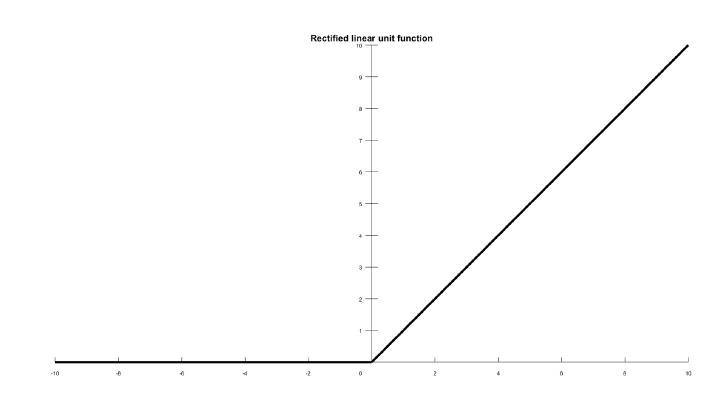
\includegraphics[width=10cm]{archivos/4.Metodologia/Modelos/CNN/RELUImage}
                    \caption{https://www.researchgate.net/journal/Transport-in-Porous-Media-1573-1634. Función ReLU}
                    \label{RELUImage}
                 \end{figure}

                La salida de la última capa de la convolución transformará el mapa de características de tamaño (\textit{5 x 5}) generada a una capa Flatten, que aplanará la matriz de tal forma que la convertirá en un vector unidimensional de (\textit{1 x 25}). A continuación se aplicará una capa densa que conectará cada uno de los \textit{25} nodos de la capa \textit{Flatten} con los \textit{128} nodos de la capa densa, que generará los logits antes de aplicar la última función de activación \textit{Softmax} que devolverá la clase predicha.


                Para ejemplificar la arquitectura de las \glsentryshort{cnn} propuestas se muestra el caso de la \glsentryshort{cnn2d} en la figura \ref{TASPCNNIMAGE}


                \begin{figure}[h]
                    \centering
                    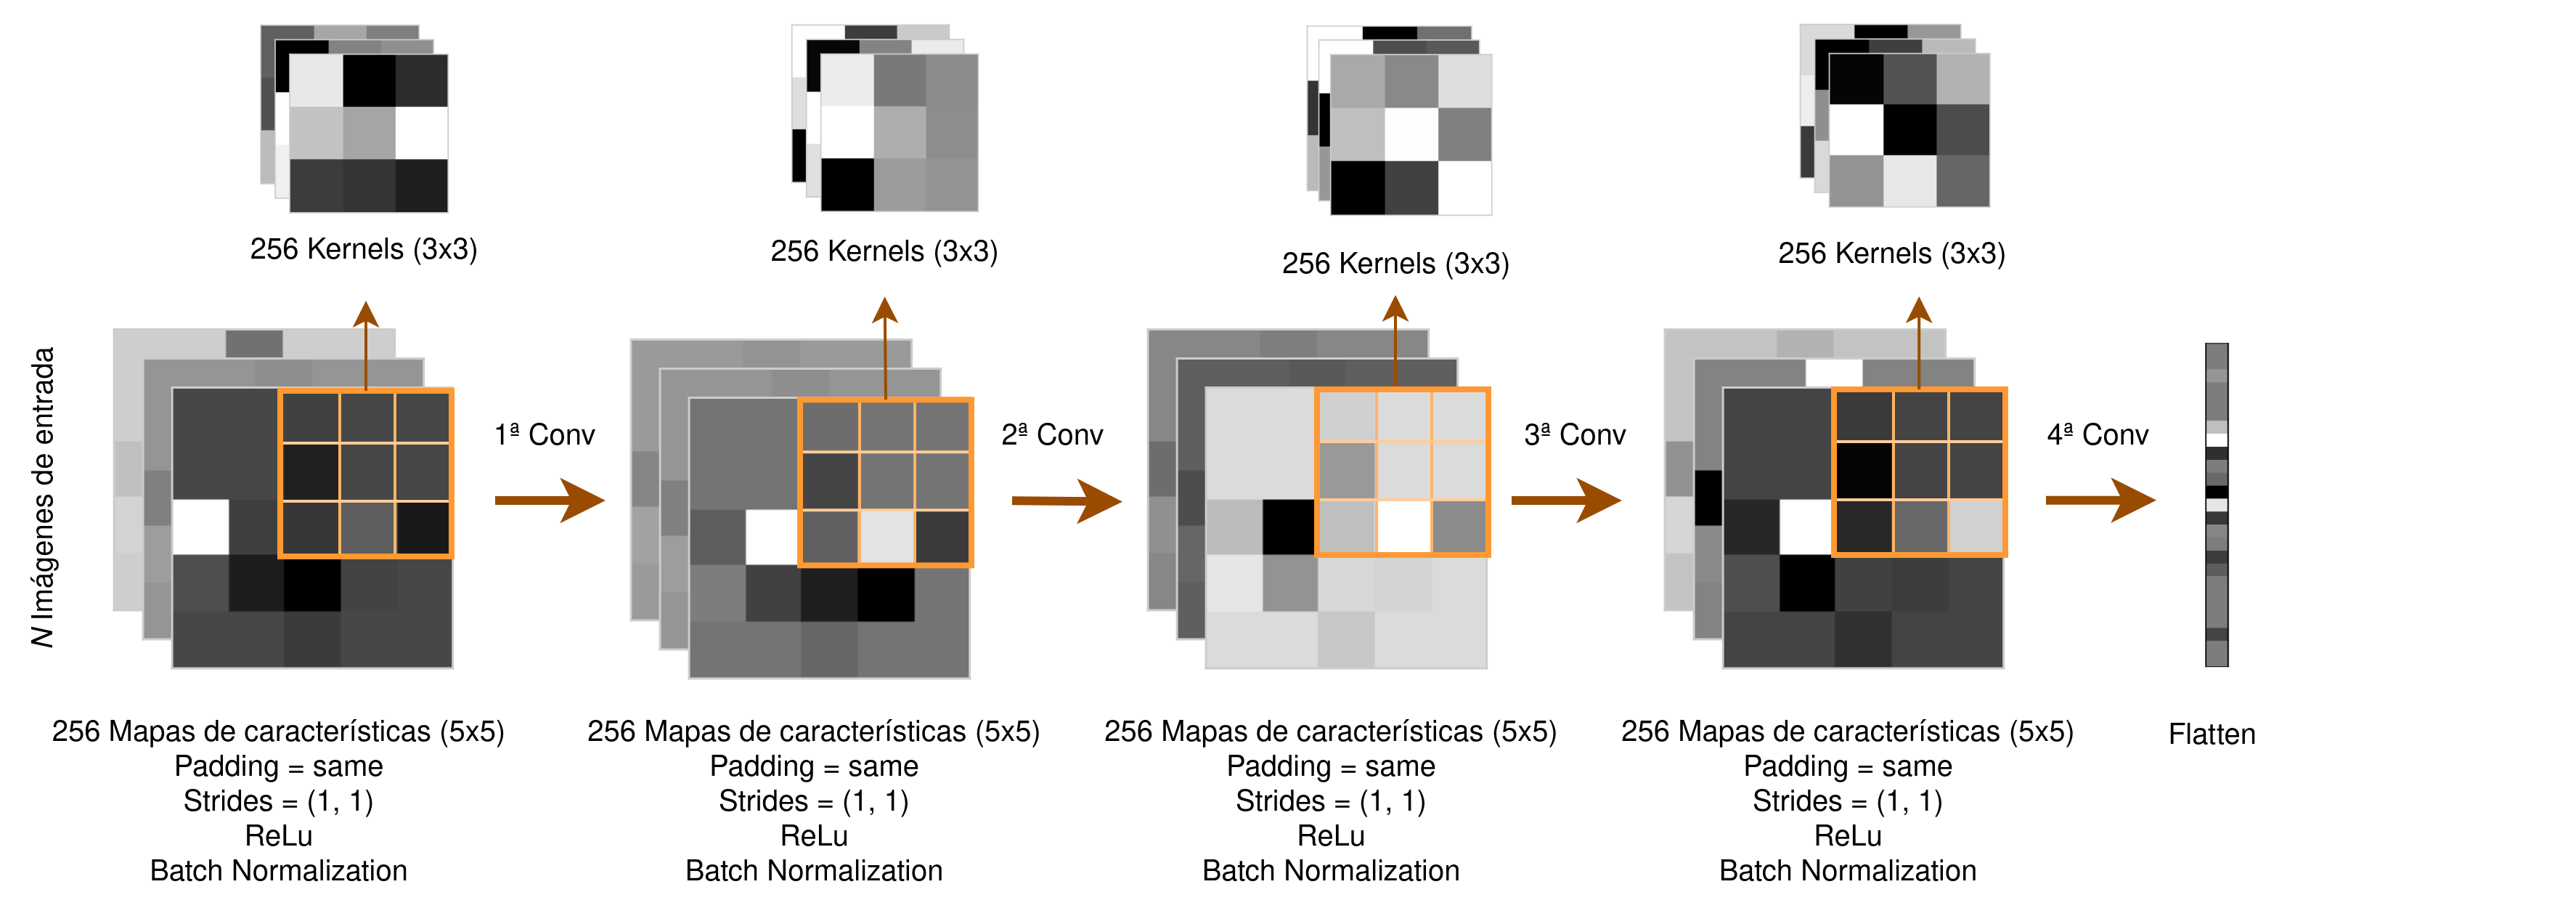
\includegraphics[width=17cm]{archivos/4.Metodologia/Modelos/CNN/2D/TASPCNN}
                    \caption{Arquitectura de la CNN-2D mostrando una  kernels aprendidos durante el entrenamiento.}
                    \label{TASPCNNIMAGE}
                 \end{figure}


        \end{enumerate}

        \cite{AutoSklearn}

\newpage
